\documentclass[default]{beamer}
\setbeamertemplate{navigation symbols}{}

\usetheme{Frankfurt}
%\useoutertheme{infolines}
\usecolortheme{beaver}

\usepackage[utf8]{inputenc}					% Выбор языка и кодировки
\usepackage[english, russian]{babel}	% Языки: русский, английский
\usepackage{csquotes}
\usepackage{tikz}
\usetikzlibrary{arrows,shapes,calc}
\usepackage{animate}
\usepackage{fp}
\usepackage{textpos}

\usepackage[
	language=auto,
	autolang=other,
	backend=biber,
	style=authortitle,
	sorting=ydnt,
	maxbibnames=5
]{biblatex}
\addbibresource{strl_cai16.bib}
				
\DeclareSourcemap{
	\maps[datatype=bibtex, overwrite]{
		\map{
			\step[fieldset=langid, fieldvalue=english]
			\step[fieldset=doi, null]
			\step[fieldset=issn, null]
			\step[fieldset=isbn, null]
			\step[fieldset=url, null]
			\step[fieldsource=language, fieldset=langid, origfieldval]
		}
	}
}
\DeclareBibliographyDriver{std}{%
	\usebibmacro{bibindex}%
	\usebibmacro{begentry}%
	\usebibmacro{author/editor+others/translator+others}%
	\setunit{\labelnamepunct}\newblock
	\usebibmacro{title}%
	\newunit\newblock
	\usebibmacro{maintitle+booktitle}
	\newunit\newblock
	\usebibmacro{journal}%
	\newunit\newblock
	\usebibmacro{date}%
	\newunit\newblock
	\usebibmacro{finentry}
}
\DeclareBibliographyAlias{article}{std}
\DeclareBibliographyAlias{book}{std}
\DeclareBibliographyAlias{inproceedings}{std}
\DeclareBibliographyAlias{incollection}{std}

\graphicspath{{../../images/}} 			% Пути к изображениям

\makeatletter
\setbeamertemplate{footline}
{
	\leavevmode%
	\hbox{%
		\begin{beamercolorbox}[wd=.333333\paperwidth,ht=2.25ex,dp=1ex,center]{author
				in head/foot}%
			\usebeamerfont{author in
				head/foot}\insertshortauthor~~\beamer@ifempty{\insertshortinstitute}{}{(\insertshortinstitute)}
		\end{beamercolorbox}%
		\begin{beamercolorbox}[wd=.333333\paperwidth,ht=2.25ex,dp=1ex,center]{title in
				head/foot}%
			\usebeamerfont{title in head/foot}\insertshorttitle
		\end{beamercolorbox}%
		\begin{beamercolorbox}[wd=.333333\paperwidth,ht=2.25ex,dp=1ex,right]{date in
				head/foot}%
			\usebeamerfont{date in head/foot}\insertshortdate{}\hspace*{2em}
			\insertframenumber{}\hspace*{2ex} 
		\end{beamercolorbox}
	}%
	\vskip0pt%
}

\renewcommand*{\bibfont}{\tiny}
\setlength\bibitemsep{-5pt}

\begin{document}
	
	\title[Направления и перспективы ИИ]{Искусственный интеллект: современное состояние и перспективы}
	\author[А.И. Панов]{\textbf{А.И. Панов}}
	\institute[ВШЭ]{НИУ ВШЭ}
	\date{Введение в методы ИИ -- 28.09.2017} 
	
	{
	\setbeamertemplate{headline}{}
	\begin{frame}
		
		\titlepage
		\centering
		\href{mailto:apanov@hse.ru}{apanov@hse.ru}
		\par\bigskip
		
\includegraphics[height=30pt]{misc/logos/ras.png} \hspace{10pt}
		
\includegraphics[height=30pt]{misc/logos/hse.png} \hspace{10pt}
		
\includegraphics[height=30pt]{misc/logos/frccsc.png} 
		
	\end{frame}
	}	

	\section{Что такое ИИ?}
	\begin{frame}
		\frametitle{Кратко о себе}
		\scriptsize
		\begin{columns}
			\begin{column}{0.85\textwidth}
				\textbf{Панов Александр Игоревич, к. ф.-м. н.}
				\begin{itemize}
					\item Старший научный сотрудник лаборатории <<Динамические интеллектуальные системы>> ИСА ФИЦ ИУ РАН.
					\item Научный сотрудник и доцент ФКН ВШЭ.
					\item Доцент кафедры системных исследований Московского физико-технического института (МФТИ).
					\item Член Российской ассоциации искусственного интеллекта (РААИ).
					\item Член Сообщества биологически инспирированных когнитивных архитектур (BICA Society).
					\item Организатор Международной конференции по биологически инспирированным когнитивным архитектурам (BICA-2016 --- Нью-Йорк, BICA-2017 --- Москва), Международной школы по биологически инспирированным когнитивным архитектурам (Fierces on BICA, Москва) и школы молодых ученых по ИИ (ISyT 2017, Санкт-Петербург).
					\item Член редколлегии журнала Biologically Inspired Cognitive Architectures.					
					\item Руководитель проектов РФФИ мол\_а, мол\_а\_дк, офи\_м.
					\item Ментор студенческой лаборатории по ИИ (SLabAI).
				\end{itemize}
			\end{column}
			
			\begin{column}{0.15\textwidth}
				\centering
				
\includegraphics[width=\textwidth]{misc/logos/ras.png}
				\vspace{7pt}
				
\includegraphics[width=\textwidth]{misc/logos/frccsc.png}
				\vspace{7pt}
				
\includegraphics[width=0.7\textwidth]{misc/logos/isa.png}
				\vspace{7pt}
				
\includegraphics[width=0.5\textwidth]{misc/logos/raai.png}
				\vspace{7pt}
				
\includegraphics[width=0.5\textwidth]{misc/logos/hse.png}
				\vspace{7pt}
				
\includegraphics[width=\textwidth]{misc/logos/mipt.jpg}
				\vspace{5pt}
				
\includegraphics[width=\textwidth]{misc/logos/BICA.png}
				\vspace{5pt}
				
\includegraphics[width=0.7\textwidth]{misc/logos/slabai3.png}
			\end{column}
			
		\end{columns}
	\end{frame}	
	\subsection{0.1}
	\begin{frame}
		\frametitle{Как себе представляют ИИ в обществе}
		\centering
		\onslide<1->{
			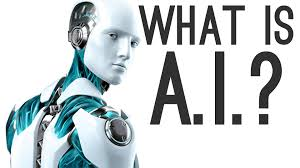
\includegraphics[width=0.3\textwidth]{ai_view0.jpg}
			\par\bigskip	
		}
		\onslide<2->{
			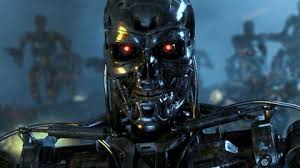
\includegraphics[width=0.3\textwidth]{ai_viewno.jpg}	
		}
		\onslide<3->{
			\begin{tikzpicture}[overlay]
			\draw[red, very thick] (-3.3,2) -- (-0.3,-0.2);
			\draw[red, very thick] (-0.3,2) -- (-3.3,-0.2);
			\end{tikzpicture}
		}
		\onslide<4->{
			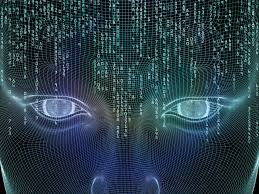
\includegraphics[width=0.3\textwidth]{ai_view1.jpg}	
		}
		\onslide<5->{
			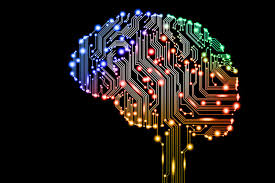
\includegraphics[width=0.3\textwidth]{ai_view2.jpg}	
			\par\bigskip
		}
		\onslide<6->{
			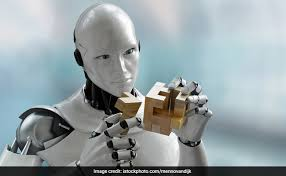
\includegraphics[width=0.3\textwidth]{ai_view5.jpg}	
		}
		\onslide<7->{
			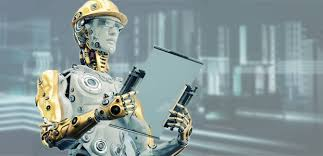
\includegraphics[width=0.3\textwidth]{ai_view3.jpg}	
		}
		\onslide<8->{
			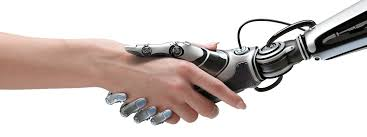
\includegraphics[width=0.3\textwidth]{ai_view4.jpg}	
		}

	
	\end{frame}

	\begin{frame}
		\frametitle{Определения ИИ}
		
		\begin{itemize}
			\onslide<1->{
				\item ИИ - это научное направление, в рамках которого ставятся и решаются задачи аппаратного или программного моделирования тех видов человеческой деятельности, которые традиционно считаются интеллектуальными (Толковый словарь по ИИ).
			}
			\onslide<2->{
				\item  ИИ - это наука и технология создания интеллектуальных машин, особенно интеллектуальных компьютерных программ (Джон Маккарти).
			}
			\onslide<3->{
				\item ИИ - это наука об <<интеллектуальных агентах>>, т.е. о некотором устройстве или программе, которая воспринимает свою среду и выполняет действия, которые максимизируют ее шансы на успех при достижении какой-то цели (Рассел и Норвиг).
			}
		\end{itemize}
	\end{frame}
	

	\begin{frame}
		\frametitle{Когнитивные науки}
		
		
		\centering
		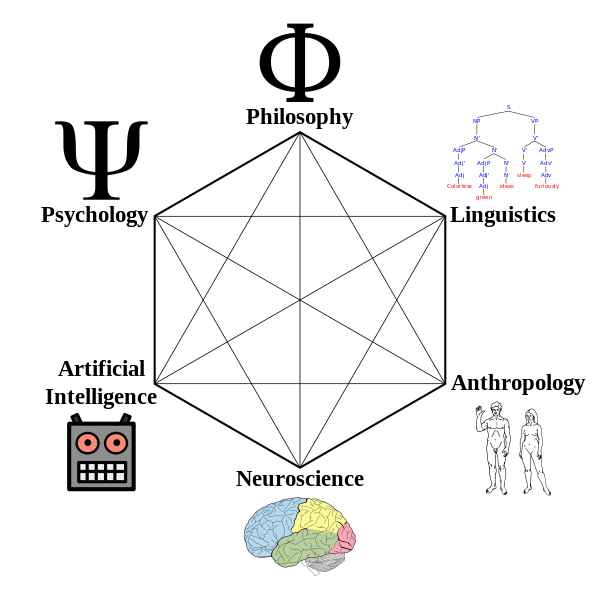
\includegraphics[width=0.5\textwidth]{cogsci.png}
		
		Когнитивная наука (лат. cognitio <<познание>>) - междисциплинарное научное направление изучающее психику, разум (mind) человека и реализующие его процессы.
	\end{frame}

	\section{Немного истории}
	\subsection{1.1}
	\begin{frame}
		\frametitle{Как это случилось}

		\begin{itemize}
			\item \textbf{1954 г.} --- аналитики \textit{Рэнд Корпорейшн}, \textit{А. Ньюэлл}, \textit{Дж. Шоу} и \textit{Г.Саймон}  решили написать программу игры в шахматы. В этой затее им вызвались помочь \textit{А. Тьюринг} и \textit{К. Шеннон}, а также группа голландских психологов.
			\item \textbf{1957 г.} --- программа для игры в шахматы (NSS) была написана. В основе работы NSS лежали эвристики --- правила выбора в отсутствие теоретических оснований.
		\end{itemize}
	\end{frame}
	\subsection{1.2}
	\begin{frame}
	\frametitle{Что произошло дальше}
	
		\begin{itemize}
			\item \textbf{1960 г.}  --- GPS (<<универсальный решатель задач>>): вычисление неопределенных интегралов, головоломки и  некоторые другие задачи.  Программы автоматического доказательства теорем из планиметрии, решения алгебраических задач. 
			\item \textbf{1960 г.} --- возникновение \textbf{эвристического программирования}. 
			\item \textbf{1963 г.} --- \textit{Джон Маккарти} --- ЛИСП. \textbf{Возникновение функционального программирования}.
		\end{itemize}
	\end{frame}
	\subsection{1.3}
	\begin{frame}
		\frametitle{Поиск непереборных методов решения задач}
		
		\begin{itemize}
			\item \textbf{1964 г.} --- \textit{В.Н. Пушкин} и \textit{Д.А. Поспелов}  --- модельная гипотеза мышления versus лабиринтной; методы решения переборных задач человеком. 
			\item \textbf{1964 г.} --- \textit{С.Ю. Маслов} --- метод автоматического поиска доказательства теорем в исчислении предикатов (обратный метод).
			\item \textbf{1965 г.} --- \textit{Дж.А. Робинсон} --- метод автоматического поиска доказательства теорем в исчислении предикатов (метод резолюций).
			\item \textbf{1968 г.} --- возникновение \textbf{логического программирования}.
			\item \textbf{1971 г.} --- \textit{А. Колменрауэр} --- \textbf{язык Пролог}.
			
		\end{itemize}
	\end{frame}

	\subsection{1.4}
	\begin{frame}
		\frametitle{Современный ИИ}
		\Large
		\begin{itemize}
			\item \textbf{Середина 70-х гг.} --- качественный скачок в работах по искусственному интеллекту.
			\item Появление  первых прикладных систем, использующих знания для решения различных всё более сложных задач.
		\end{itemize}
	\end{frame}

	\begin{frame}
	\frametitle{Современный ИИ}
		\centering
		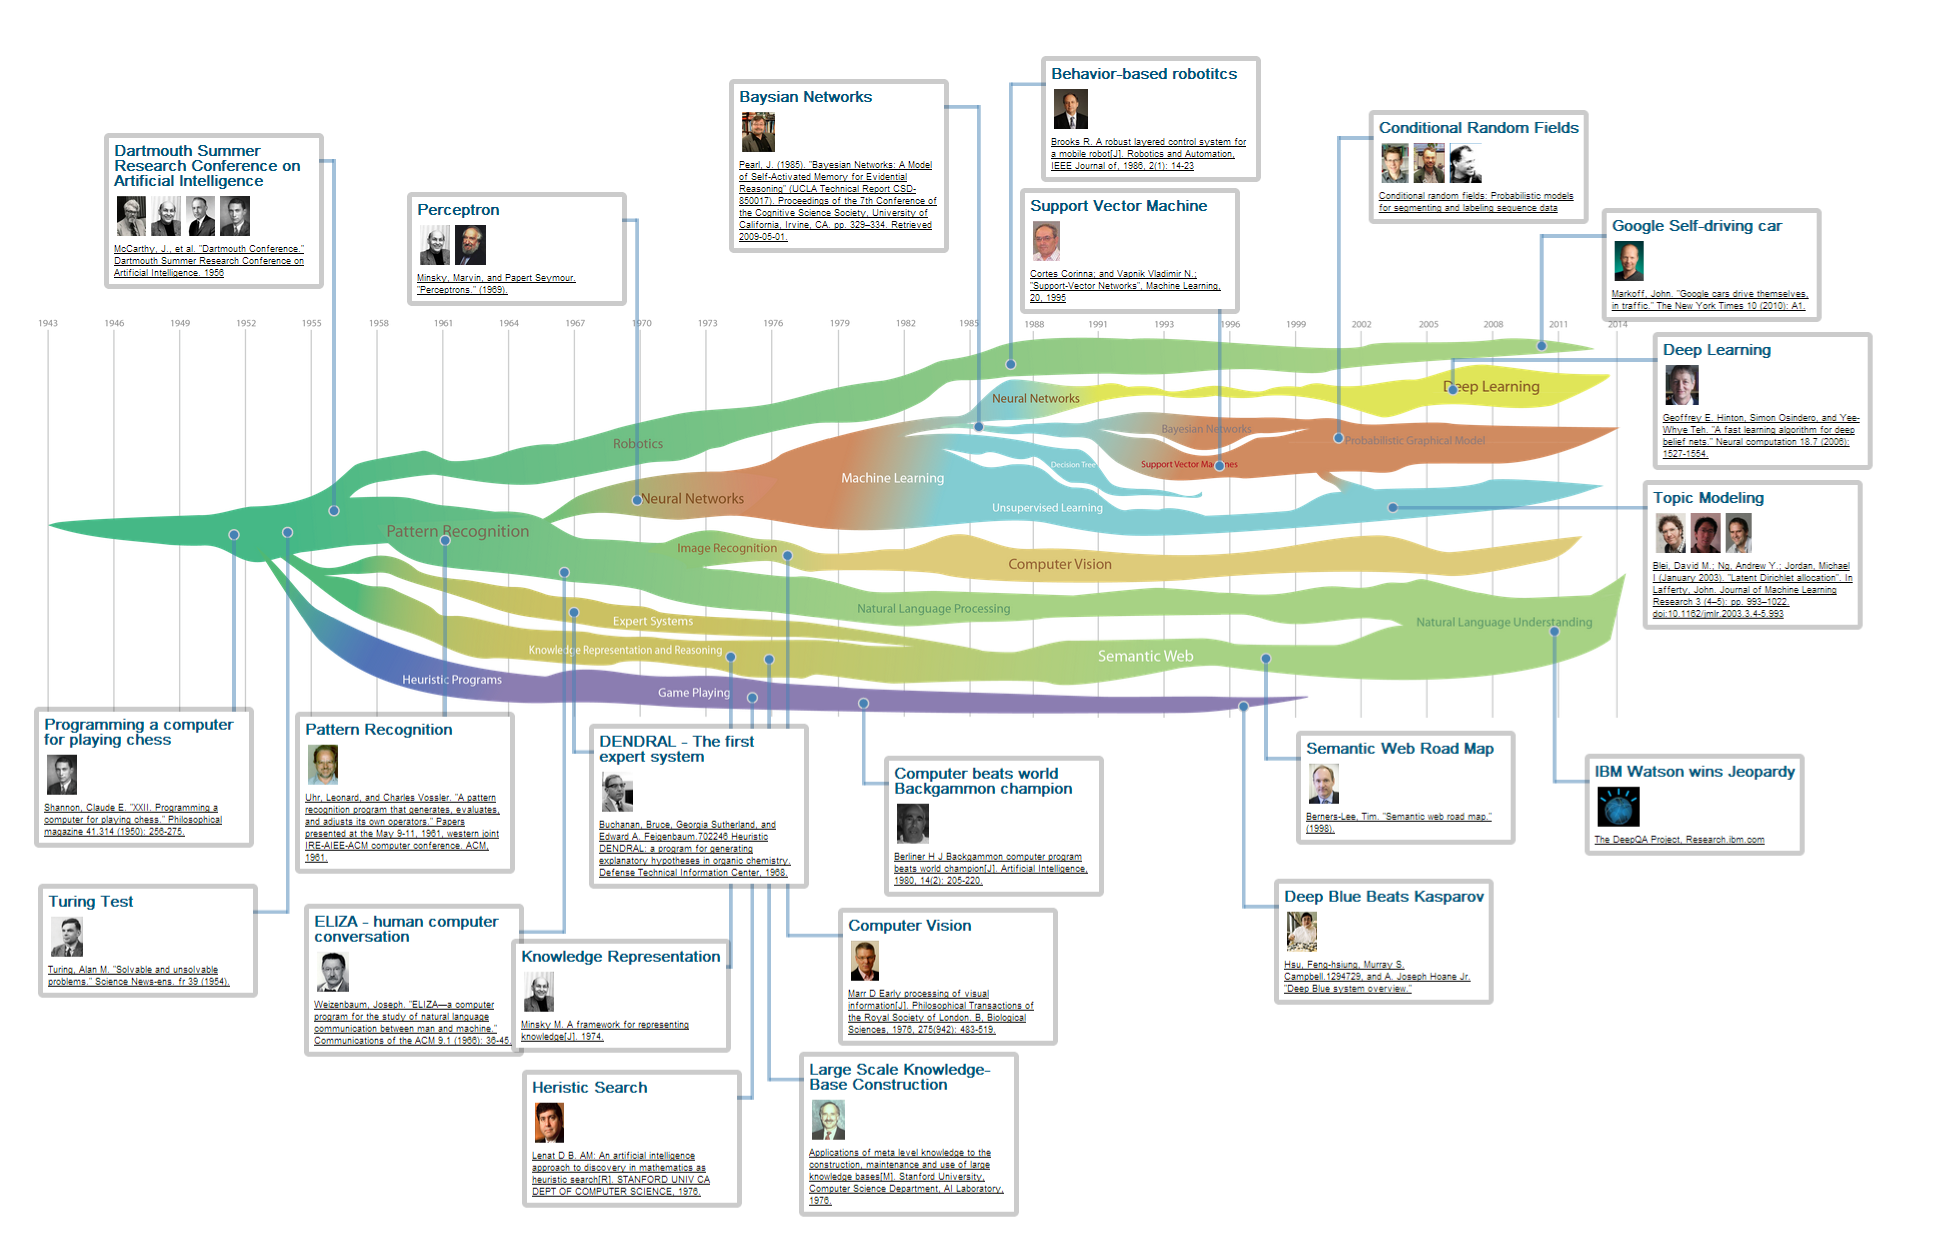
\includegraphics[width=\textwidth]{ai-1.png}
	\end{frame}

	\section{Организация ИИ}
	\subsection{2.1}
	\begin{frame}
		\frametitle{Искусственный интеллект --- организационная структура}
		
		\begin{itemize}
			\item Во многих странах есть ассоциации искусственного интеллекта (EurAI,AAAI, RAAI).
			\item Каждый или раз в два года проходят крупнейшие конференции по ИИ: ECAI, AAAI Conference, IJCAI, КИИ.
			\item РААИ - общероссийская общественная организация (261 индивидуальный член, 45 региональных отделений).
			\item Выходят тематические журналы (Artificial Intelligence, Cognitive Psychology, Autonomous Robots, Neural Networks, Искусственный интеллект и принятие решений).
		\end{itemize}
		\par\bigskip
		\centering
		
\includegraphics[height=30pt]{aaai.png} \hspace{10pt}
		
\includegraphics[height=30pt]{eurai.png} \hspace{10pt}
		
\includegraphics[height=30pt]{misc/logos/raai.png} 
	\end{frame}

	\subsection{2.2}
	\begin{frame}
		\frametitle{Источники}
		\scriptsize
		Онлайн: Coursera, Udacity, postnauka.ru, курсы ведущих университетов:
				\begin{itemize}
					\item Machine Learning and Artificial Intelligence в Принстоне (\url{https://www.cs.princeton.edu/courses/archive/fall16/cos402/})
					\item Artificial Intelligence в CMU (\url{http://www.cs.cmu.edu/~./15381/})
					\item Deep Learning for Self-Driving Cars в MIT (\url{http://selfdrivingcars.mit.edu})
					\item Deep Reinforcement Learning в Беркли (\url{http://rll.berkeley.edu/deeprlcourse/})
				\end{itemize}
		Книги:
			\begin{itemize}
				\item  Nilsson N.J. Artificial Intelligence: A New Synthesis. San Francisco: Morgan Kaufmann, 1998. 513 p.
				\item Russell S., Norvig P. Artificial Intelligence: A Modern Approach, Prentice Hall, 2009 (3 edition), P. 1152. (Искусственный интеллект. Современный подход)
				\item Осипов Г.С. Методы искусственного интеллекта. М.: ФИЗМАТЛИТ, 2011.
				\item Flreani D., Mattiussi C. Bio-Inspired Artificial Intelligence: Theories, Methods, and Technologies, The MIT Press, 2008, P. 658.
				\item Поспелов Д.А. Моделирование рассуждений. Опыт анализа мыслительных актов. М.: Радио и связь, 1989. 184 с.
				\item Гаазе-Рапопорт М.Г., Поспелов Д.А. От амебы до робота. Модели поведения. М.: Наука, 1987. 288 с.
				\item Что-то <<популярное>> (Джефф Хокинс, Сандра Блейксли. Об интеллекте; Роджер Пенроуз. Новый ум короля)
			\end{itemize}
	   Профессиональные интернет-ресурсы (\url{http://open.ai}, \url{https://deepmind.com})
	\end{frame}


	\section{Направления ИИ}
	\subsection{3.1}
	\begin{frame}
		\frametitle{Основные направления ИИ}
		\centering
		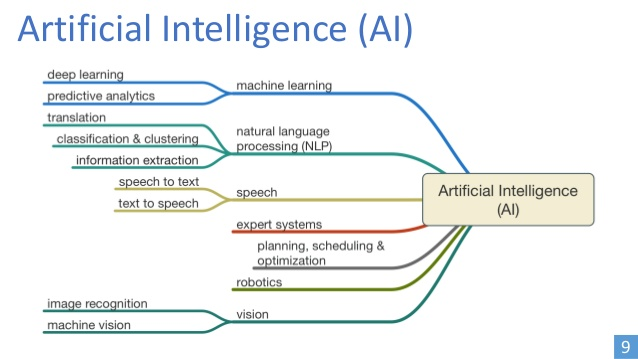
\includegraphics[width=\textwidth]{ai_fields.jpg}
	\end{frame}

	\begin{frame}
		\frametitle{Основные направления ИИ}
		\centering
		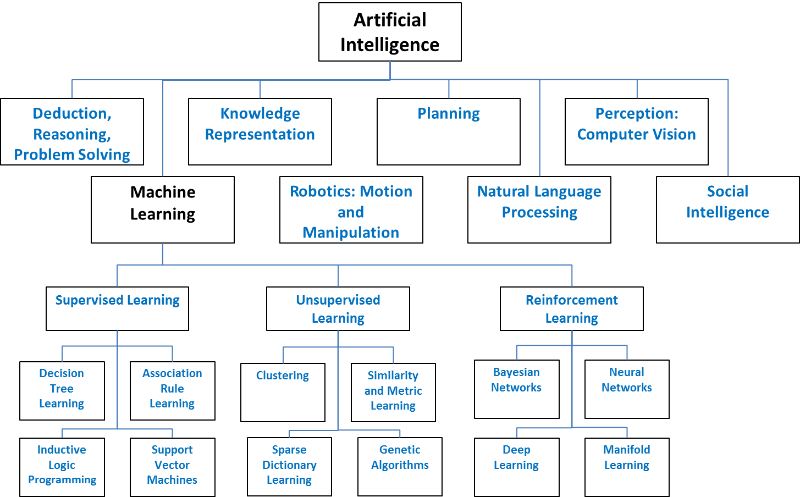
\includegraphics[width=\textwidth]{ai_fields3.png}
	\end{frame}

	\begin{frame}
		\frametitle{Основные направления ИИ}
		\centering
		\footnotesize
		\makebox[0.8\textwidth][c]{
			\begin{tikzpicture}
				\node[ellipse, minimum width = 100, minimum height = 50, fill=blue!20, align=center] (d1) {Искусственный\\интеллект};
				
				\node[rounded corners=5pt,draw,color=blue!20, very thick,text=black] (d2) at (-4,2) {
					\begin{minipage}[c][33pt]{100pt}
						\centering
						\textbf{Приобретение знаний, анализ данных и порождение гипотез}
					\end{minipage}
				};
				\node[rounded corners=5pt,draw,color=blue!20, very thick,text=black] (d3) at (-4,0.5) {
					\begin{minipage}[c][20pt]{80pt}
					\centering
					\textbf{Моделирование рассуждений}
					\end{minipage}
				};
	
				\node[rounded corners=5pt,draw,color=blue!20, very thick,text=black] (d4) at (-4,-0.7) {
					\begin{minipage}[c][20pt]{80pt}
					\centering
					\textbf{Многоагентные системы}
					\end{minipage}
				};
			
				\node[rounded corners=5pt,draw,color=blue!20, very thick,text=black] (d5) at (-4,-2.3) {
					\begin{minipage}[c][43pt]{110pt}
					\centering
					\textbf{Обработка естественного языка, пользовательский интерфейс и модели пользователя}
					\end{minipage}
				};
			
			
				\node[rounded corners=5pt,draw,color=blue!20, very thick,text=black] (d6) at (4,2) {
					\begin{minipage}[c][33pt]{120pt}
					\centering
					\textbf{Динамические интеллектуальные системы и планирование поведения}
					\end{minipage}
				};
				\node[rounded corners=5pt,draw,color=blue!20, very thick,text=black] (d7) at (4,0.5) {
					\begin{minipage}[c][20pt]{80pt}
					\centering
					\textbf{Представление знаний}
					\end{minipage}
				};
				
				\node[rounded corners=5pt,draw,color=blue!20, very thick,text=black] (d8) at (4,-0.7) {
					\begin{minipage}[c][20pt]{100pt}
					\centering
					\textbf{Нечеткие модели и мягкие вычисления}
					\end{minipage}
				};
				
				\node[rounded corners=5pt,draw,color=blue!20, very thick,text=black] (d9) at (4,-2.3) {
					\begin{minipage}[t][20pt]{110pt}
					\centering
					\textbf{Инструментальные средства и технологии}
					\end{minipage}
				};
				
				\draw[->,rounded corners=10pt, very thick, blue!20](d1)[xshift=-10] |- (d2.east);
				\draw[->,rounded corners=10pt, very thick, blue!20](d1)[xshift=10] |- (d6.west);
				
				\draw[->,rounded corners=10pt, very thick, blue!20](d1)[xshift=-10] |- (d5.east);
				\draw[->,rounded corners=10pt, very thick, blue!20](d1)[xshift=10] |- (d9.west);
				
				\draw[->,rounded corners=10pt, very thick, blue!20](d1) |- (d3.east);
				\draw[->,rounded corners=10pt, very thick, blue!20](d1) |- (d7.west);
				
				\draw[->,rounded corners=10pt, very thick, blue!20](d1.south west) |- (d8.west);
				\draw[->,rounded corners=10pt, very thick, blue!20](d1.south east) |- (d4.east);
			\end{tikzpicture}
		}
	\end{frame}

	\subsection{3.2}
	\begin{frame}
		\frametitle{Приобретение знаний, анализ данных и автоматическое порождение гипотез}
		
		\textbf{Цель}: создание методологий, технологий и программных средств обнаружения и переноса компетентности   в базы знаний.
		\par\medskip
		\centering
		\tikz[baseline]{
			\small
			\node[fill=yellow, rounded corners=5pt, minimum width=300, minimum height = 150] (k1) {
				\begin{minipage}[t][150pt]{300pt}
					\centering
					\textbf{Методы приобретения знаний:}
				\end{minipage}
				
			};
			
			\node[rounded corners=5pt, minimum width=280, minimum height = 50, text width= 250, text centered,fill=white] (k2) at (0, 0.85) {
				\begin{minipage}[t][60pt]{250pt}
					\centering
					\textbf{Машинное обучение и обучение по примерам} (методы построения деревьев решений,  индуктивные методы построения правил;  статистические методы, в частности, Байесовские  сети; метод ближайших соседей, искусственные нейронные сети)
				\end{minipage}
				
			};
		
			\node[rounded corners=5pt, minimum width=280, minimum height = 10, text width= 250, text centered,fill=white] (k2) at (0,-0.9) {
				\begin{minipage}[t][10pt]{250pt}
					\centering
					\textbf{Приобретение знаний из текстов}
				\end{minipage}
				
			};
		
			\node[rounded corners=5pt, minimum width=280, minimum height = 20, text width= 250, text centered,fill=white] (k2) at (0, -2) {
				\begin{minipage}[t][20pt]{250pt}
					\centering
					\textbf{Прямые методы приобретения знаний (автоматизированный диалог с экспертами)}
				\end{minipage}
				
			};
		}
	\end{frame}

	\subsection{3.3}
	\begin{frame}
		\frametitle{Представление знаний}
		
		\textbf{Предмет}:  разработка языков и программных средств   для описания экспертных и эмпирических знаний. 
		\par\medskip
		\textbf{Содержание}:
		\begin{itemize}
			\item семантические сети, системы фреймов, системы правил (продукционные системы) и их гибриды;
			\item логики пространства и времени;
			\item онтологии – способ обмена знаниями;
			\item дескриптивные логики (теория баз знаний и онтологий).
		\end{itemize}
	\end{frame}

	\subsection{3.4}
	\begin{frame}
		\frametitle{Автоматизация  рассуждений}
		
		Методы индукции, абдукции и аналогии, аргументации, рассуждения на основе прецедентов, на основе ограничений, рассуждения о действиях и изменениях, рассуждения с неопределенностью, немонотонные рассуждения.
		\par\medskip
		\tikz[baseline]{
			\node[fill=blue!20, rounded corners=5pt, anchor=base] (t1) {\textbf{Немонотонные рассуждения}};
		}
		связаны с поиском эмпирических зависимостей в данных, обучением по примерам и рассуждениями в эмпирических  теориях. Выделились в самостоятельный раздел логики.
		\par\medskip
		\tikz[baseline]{
			\node[fill=blue!20, rounded corners=5pt, anchor=base] (t2) {\textbf{Рассуждения о действиях}};
		}
		исследуют связь  действий и эффектов действий (результатов действий).
		\par\medskip
		\tikz[baseline]{
			\node[fill=blue!20, rounded corners=5pt, anchor=base] (t3) {\textbf{Рассуждения с неопределенностью}};
		}
		--- использование  Байесовского  формализма в моделях рассуждений. 
		
	\end{frame}

	\subsection{3.5}
	\begin{frame}
		\frametitle{Многоагентные системы}
		
		Изучаются интеллектуальные программные агенты, их коалиции и поведение.
		
		\par\medskip
		\textbf{Интеллектуальный программный  агент} --- программная система, обладающая автономностью, социальными чертами, реактивностью и активностью.
		
		\par\medskip
		\textbf{Основные проблемы}: коммуникация интеллектуальных агентов, разработка языков для этой цели, координация поведения  агентов, распределение ролей в коалициях агентов, коллективное поведение агентов.
	\end{frame}

	\subsection{3.7}
	\begin{frame}
		\frametitle{Роботы и автономные системы}
		\Large
		\begin{itemize}
			\item Диалоговое взаимодействие коалиций мобильных роботов.
			\item Интерпретация команд, поступающих от человека.
			
			\item Качественные логики пространства-времени.
			
			\item Рассуждения, основанные на оценках.
			
			\item Проблема символизации (symbol grounding problem).
		\end{itemize}
		
	\end{frame}

	\subsection{3.8}
	\begin{frame}
		\frametitle{Интеллектуальные динамические системы и автоматическое планирование поведения}
		\Large
		
		\textbf{Результат интеграции} методов искусственного интеллекта с теорией динамических систем:
		\begin{itemize}
			\item планирование,
			\item моделирование,
			\item управление.
		\end{itemize}
		
	\end{frame}

	%\subsection{3.9}
	\begin{frame}
		\frametitle{Обработка естественного языка, интерфейс и модели пользователя}
		\begin{itemize}
			\small
			\item Семантический поиск в больших массивах текстов:
			\begin{itemize}
				\footnotesize
				\item поиск документов (в полнотекстовой БД, в локальных и глобальных телекоммуникационных сетях);
				\item извлечение данных из текстов;
				извлечение знаний из текстов.
			\end{itemize}
			
			\item Обработка текстов: сегментация, классификация, кластеризация, аннотирование или реферирование текстов. Перевод. 
			\item Диалоговые системы: 
			\begin{itemize}
				\footnotesize
				\item интеллектуальные вопросно-ответные системы; 
				\item системы общения конечных пользователей с БД, предоставляющие  различные услуги (выполнение банковских операций по телефону, заказ товаров по каталогам); 
				\item голосовое управление техникой, кооперативное решение проблем (человек плюс интеллектуальная система).
			\end{itemize}
			
			\item Автоматическое обучение анализу текстов.
			
		\end{itemize}
		
	\end{frame}

	\subsection{3.10}
	\begin{frame}
		\frametitle{Нечеткие модели и мягкие вычисления}
		
		\Large 
		\begin{itemize}
			\item Нечеткие схемы вывода по аналогии;
			\item теория нечетких мер; 
			\item модели геометрических объектов;
			\item алгоритмы эволюционного моделирования с динамическими параметрами (например, время жизни и размер популяции);
			\item методы решения оптимизационных задач с использованием технологий генетического поиска, гомеостатических и синергетических принципов и элементов самоорганизации. 
		\end{itemize}
		
	\end{frame}

	\subsection{3.11}
	\begin{frame}
		\frametitle{Вклад ИИ в другие  науки}
		
		Развитие ИИ привело к \textbf{возникновению самостоятельных областей}:
		\begin{itemize}
			\item эвристическое программирование,
			\item функциональное программирование,
			\item логическое программирование,
			\item объектно-ориентированное программирование,
			\item теория немонотонных рассуждений и немонотонные логики,
			\item инженерия знаний,
			\item технология программирования, основанная на знаниях,
			\item прикладная семиотика.
		\end{itemize}
		
		В \textbf{инженерном направлении}:
		\begin{itemize}
			\item экспертные системы.
		\end{itemize}
	\end{frame}

	\section{Перспективы ИИ}
	\subsection{4.1}
	\begin{frame}
		\frametitle{Перспективные направления ИИ}
		
		\begin{itemize}
			\item \textbf{Рассуждения, основанные на прецедентах}.
			\item \textbf{Рассуждения о пространстве} --- возрастающее значение для автономных мобильных устройств, анализа изображений (в частности, аэрофотоснимков), синтеза текстовых описаний по изображениям.
			\item \textbf{Методы машинного обучения и автоматического формирования гипотез} --- решение практических задач: от обнаружения  закономерностей в данных до повышения степени адаптивности различных технических устройств.
			\item Подходы, основанные на \textbf{технологии интеллектуальных агентов} перспективны при разработке больших программных систем.
			
		\end{itemize}
		
	\end{frame}

	\subsection{4.2}
	\begin{frame}
		\frametitle{Перспективные направления ИИ}
		
		\begin{itemize}
			\item \textbf{Влияние идей и методов ИИ на машинный анализ текстов на естественном языке} --- коснется  семантического анализа и методов синтаксического анализа --- в этой области оно проявится в учете модели мира и использовании знаний о предметной области  для уменьшения переборов  на более ранних стадиях анализа.
			\item \textbf{Понимание текста}.
			\item \textbf{Автоматическое планирование и управление поведением}. Область применения  - от бытовой  техники до беспилотных аппаратов для исследования глубокого космоса.
		\end{itemize}
		
	\end{frame}

	\subsection{4.4}
	\begin{frame}
		\frametitle{Проблемы}
		
		\begin{itemize}
			\item Переход от моделирования структурной организации к моделированию ментальных представлений, в частности, когнитивных функций, иначе говоря,от искусственного интеллекта --- к искусственному сознанию.
			\item Автоматическое (или полуавтоматическое) формирование интеллектуальными агентами модели мира, включая зрительные и слуховые образы предметов и их назначение.

		\end{itemize}
		
	\end{frame}

	\section{Прикладной ИИ}
	\subsection{5.1}
	\begin{frame}
		\frametitle{ИИ в индустрии}
		\centering
		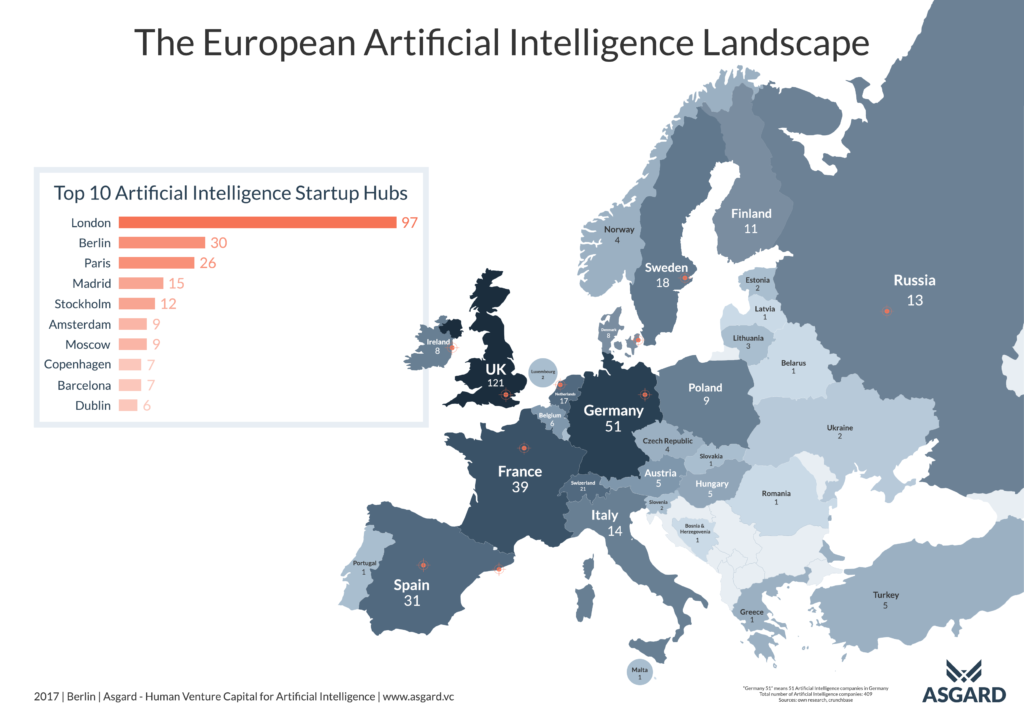
\includegraphics[width=0.6\textwidth]{asgard_1.png}
		\par\bigskip
		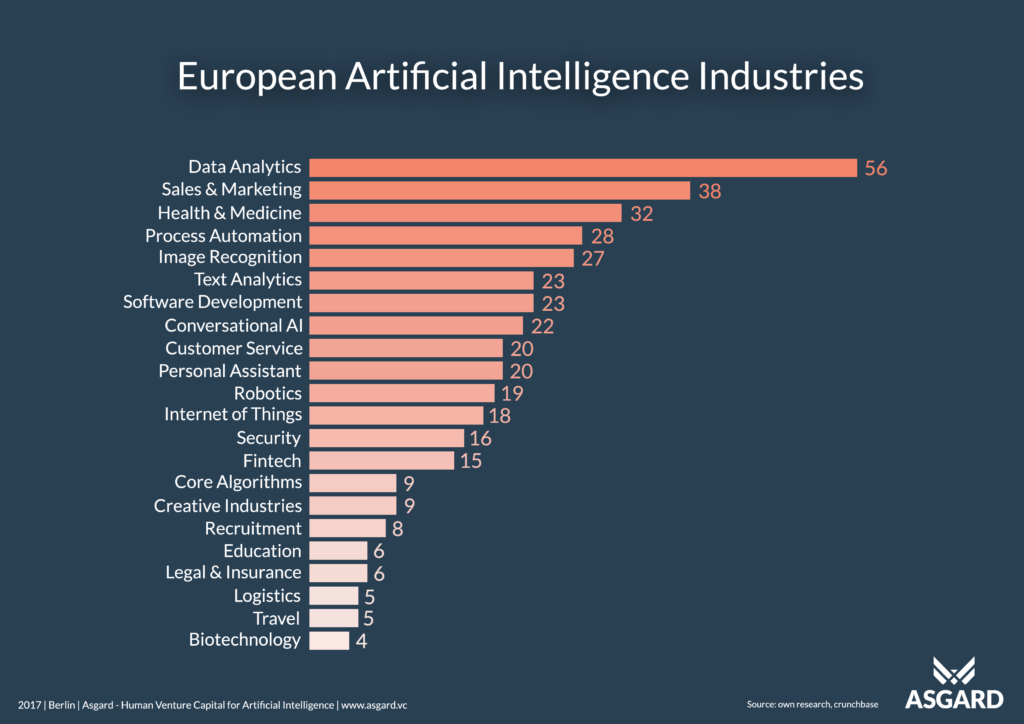
\includegraphics[width=0.3\textwidth]{asgard_2.png}
	\end{frame}

	\begin{frame}
		\frametitle{ИИ стартапы}
		\centering
		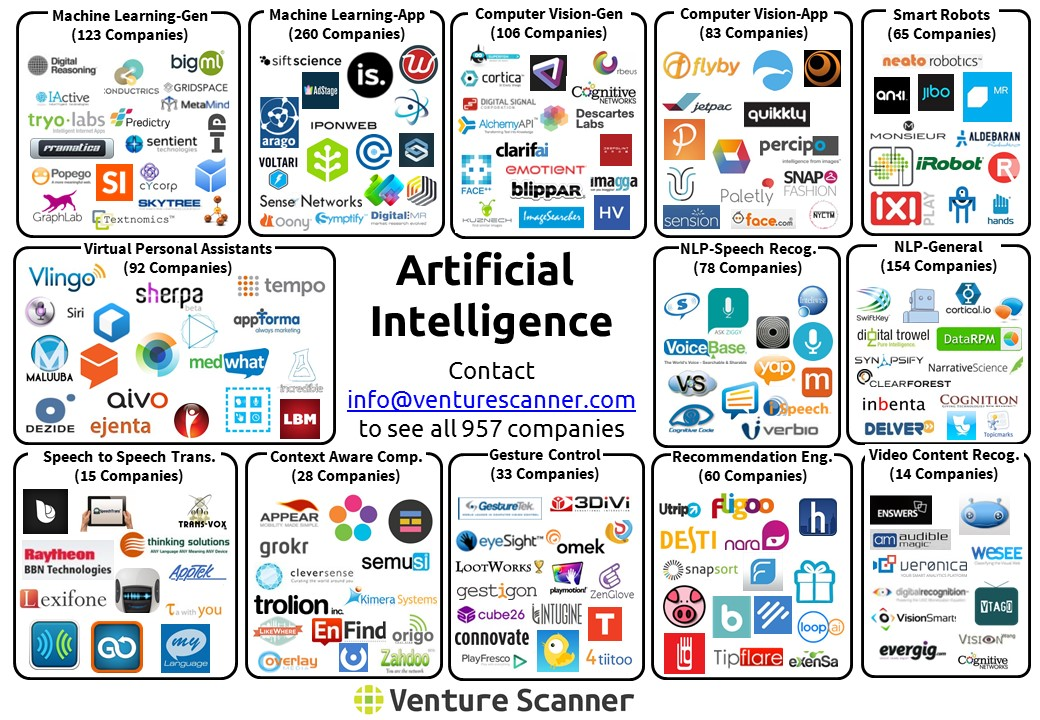
\includegraphics[width=\textwidth]{ai_startups.jpg}
	\end{frame}

	\begin{frame}
		\frametitle{Финансирование ИИ}
		\centering
		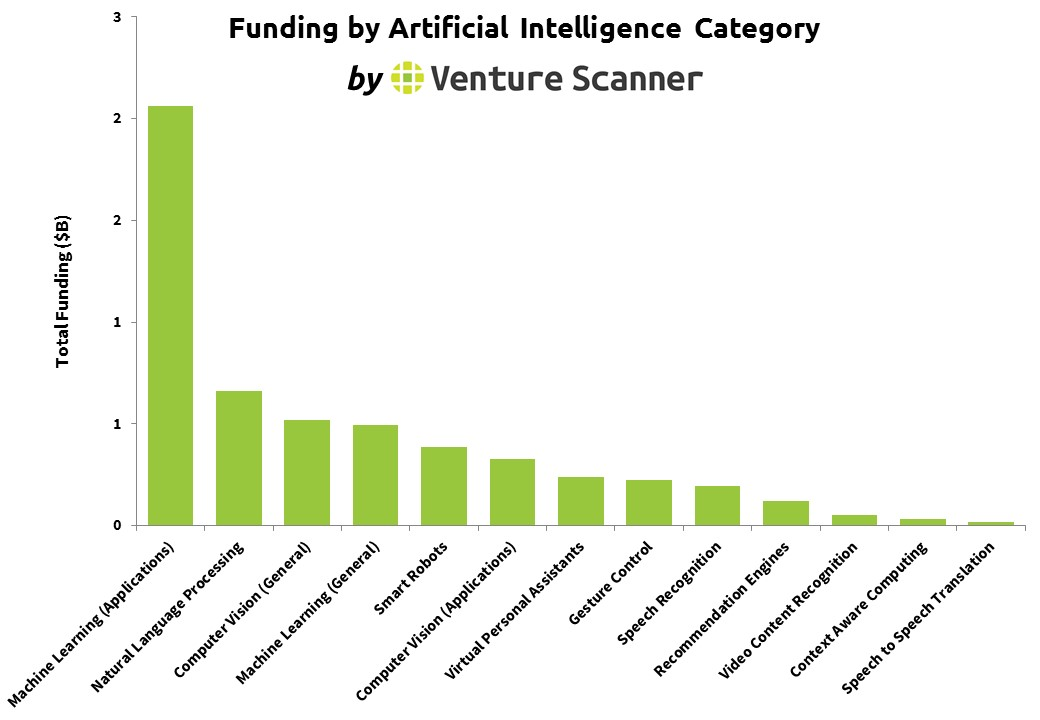
\includegraphics[width=0.7\textwidth]{ai_fund.jpg}
	\end{frame}

	\subsection{5.2}
	\begin{frame}
		\frametitle{Некоторые результаты в России}

		\begin{itemize}
			\item Разработан комплекс моделей поддержки принятия решений в конфликтных ситуациях с использованием когнитивных карт (ИПУ РАН). 
			\item Для модели летательного аппарата <<Этап>>	разработана теория бортовых 	интеллектуальных систем тактического уровня (БИС-Т/У), решающих задачи оперативного целеполагания и конструирования способа достижения оперативно назначенной цели (ГосНИИАС).
			\item Созданы роботы, архитектура системы управления которых включает эмоциональную компоненту (НИЦ <<Курчатовский институт>>). 
			\item Разработаны технологии поддержки интеллектуальных роботов-манипуляторов, способных автоматически принимать решения непосредственно во время работы (ИПМ РАН).
		\end{itemize}
	\end{frame}

	\begin{frame}
		\frametitle{Некоторые результаты в ФИЦ ИУ РАН}
		
		\begin{itemize}
			\item Создана семантическая поисковая машина нового поколения EXACTUS.  Машина работает с запросами на естественном языке.
			\item Неоднократно занимала первые места по релевантности поиска на соревнованиях поисковых 	машин \href{www.exactus.ru}{www.exactus.ru}.
			\item Создана система прогнозирования социального стресса на основе анализа социальных медиа.
			\item Созданы системы
			\begin{itemize}
				\item EXACTUS EXPERT --- для cемантического поиска и анализа качества научных публикаций,
				\item EXACTUS PATENT --- для семантического поиска и анализа патентной информации.
				\item EXACTUS LIKE для обнаружения близких текстов и вычисления степени семантической близости;
				\item TEXT Appliance --- информационно-аналитическая система анализа неструктурированной информации.
			\end{itemize}
		\end{itemize}
	\end{frame}

	\begin{frame}
		\frametitle{Сильные коллективы в России}
		
		\begin{itemize}
			\item Кузнецов С.О. (ВШЭ),
			\item Ветров Д.П. (ВШЭ),
			\item Кузнецов О.П. (ИПУ РАН)
			\item Воронцов К.В. (ВЦ РАН),
			\item Тулупьев А.В. (СПИИ РАН),
			\item Бурцев М.В. (МФТИ),
			\item Осипов Г.С. (ИСА РАН).
		\end{itemize}
	\end{frame}
	\section*{}
	{
	\setbeamertemplate{headline}{}
	\begin{frame}
		\centering
		\Huge
		Спасибо за внимание!
		\normalsize
		\par\bigskip
		\par\bigskip
		НИУ ВШЭ
		
		\par\bigskip
		apanov@hse.ru
	\end{frame}			
	}
\end{document}
	
	
